\section{Планирование для непрерывного управления}\label{lqrsection}

\subsection{Differentiable Dynamic Programming (DDP)}

% Чтобы добить читателя окончательно, займёмся оптимальным управлением. Единственное отличие будет заключаться в том, что мы посмотрим на задачу с дискретным временем, поэтому вместо дифференциального уравнения в качестве модели мира у нас будет просто $s' = f(s, a)$.

Построим планировщик для непрерывных пространств действий. Предположим, что модель динамики среды и награды (то есть все функции из постановки задачи) нам известны, причём даны не просто как симулятор, а как дифференцируемые и, главное, детерминированные функции. Для упрощения повествования будем считать, что эпизод состоит из $T$ шагов. Дополнительно рассматривая случай непрерывного пространства действий $\A \equiv \R^d$, мы получим ситуацию, в которой мы можем просто дифференцировать вдоль оси времени и оптимизировать награду по действиям <<напрямую>>.

В силу детерминированности функции переходов наш выбор действий полностью определяет траекторию. То есть искать будем даже не оптимальную детерминированную стратегию, а \emph{оптимальное управление} --- набор действий $a_1, a_2 \dots a_T$, которые приведут к наилучшей траектории. 

Поскольку мы здесь немного уходим в мир оптимального управления, поэтому для соблюдения каноничности не будем предполагать однородность: функции награды и динамики среды дополнительно зависят от дискретной переменной времени $t \in \{0 \dots T\}$. 

Итого, рассматриваем следующую задачу:
\begin{equation}\label{LQRtask}
\begin{cases}
\sum_t^T r_t(s_t, a_t) \to \max\limits_{a_1 \dots a_T} \\
s_t = f_t(s_{t-1}, a_{t-1})
\end{cases}
\end{equation}

Сразу заметим, что при сделанных предположениях можно попытаться решать задачу <<в лоб>>. Промоделируем стратегию детерминированной нейросеткой $\pi_t(s, \theta)$ с параметрами $\theta$, и рассмотрим такой вычислительный граф:

\begin{center}
    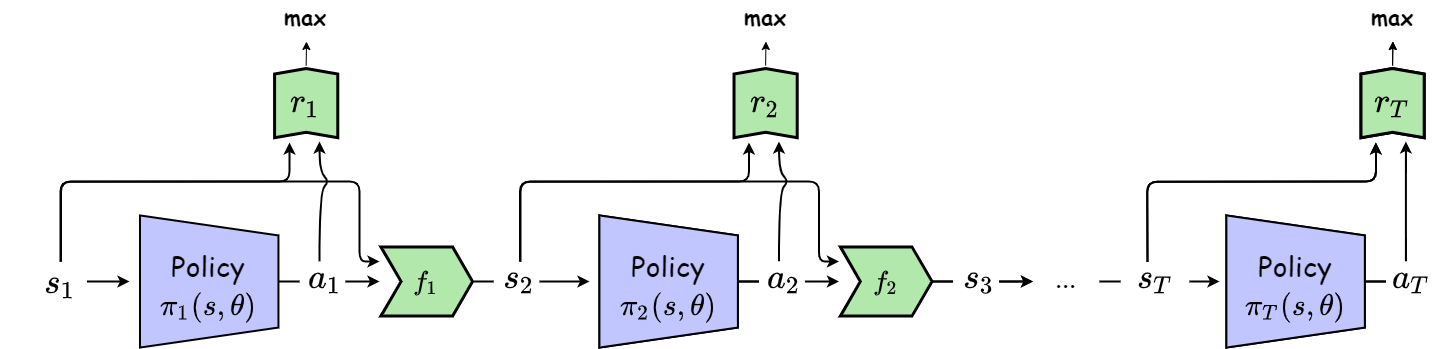
\includegraphics[width=\textwidth]{Images/DDP.png}
\end{center}

Здесь суммарная награда --- дифференцируемая функция от $\theta$, поэтому параметры стратегии можно оптимизировать напрямую. Таким образом, у нас получилась <<дифференцируемая>> задача динамического программирования. Однако, если $T$ велико, то градиент вдоль такого вычислительного графа будет подвержен затуханию, а сам такой поиск в пространстве траектории будет содержать множество локальных минимумов.

\subsection{Linear Quadratic Regulator (LQR)}

Пусть функция $f$ --- линейна, функция $r$ --- квадратична (hence the name). Введём соответствующие обозначения:
\begin{equation}\label{lineardynamics}
f_t(s, a) = F_t \begin{bmatrix} s \\ a \end{bmatrix} + f_t
\end{equation}
$$r_t(s, a) = \frac{1}{2} \begin{bmatrix} s \\ a \end{bmatrix}^T R_t \begin{bmatrix} s \\ a \end{bmatrix} + \begin{bmatrix} s \\ a \end{bmatrix}^T r_t$$

Напоминаем, что выход функции $f$ --- следующее состояние (т.е. вектор), поэтому $F_t$ --- матрица, $f_t$ --- вектор. Выход функции $r$ --- скаляр, поэтому $R_t$ --- матрица, $r_t$ --- вектор. Свободный член квадратичной формы не пишем, потому что он не зависит от состояний и действий (траектории), поэтому при оптимизации это константная неоптимизируемая награда, и она несущественна. Матрицы $F_t, R_t$ и вектора $r_t, f_t$ считаем известными. 

Нам понадобится ещё чуть-чуть обозначений. Будем считать, что блоки матрицы $R_t$ и блоки вектора $r_t$ выглядят следующим образом:
$$R_t \coloneqq \begin{bmatrix} R_{t, s, s} & R_{t, s, a} \\ R_{t, a, s} & R_{t, a, a} \end{bmatrix}; \qquad r_t \coloneqq \begin{bmatrix} r_{t, s} \\ r_{t, a} \end{bmatrix}$$

Поймём, что мы можем решить задачу обычным динамическим программированием <<с конца>>.
\begin{theorem}
Оптимальное действие в последний момент времени $a_T^*$ --- линейная форма от состояния $s_T$.
\begin{proof}
Рассмотрим последний момент времени $T$ и распишем оптимальную Q-функцию (в силу отказа от однородности оценочные функции также зависят от времени):
$$Q^*_T(s_T, a_T) = r_T(s_T, a_T) = \frac{1}{2} \begin{bmatrix} s_T \\ a_T \end{bmatrix}^T R_T \begin{bmatrix} s_T \\ a_T \end{bmatrix} + \begin{bmatrix} s_T \\ a_T \end{bmatrix}^T r_T$$

И всё, потому что на сим эпизод заканчивается и награды больше не будет. Мы легко можем найти оптимальное действие, если на последнем шаге оказались в состоянии $s_T$, промаксимизировав $Q^*_T$ по действию $a_T$:
$$a^*_T = \argmax_{a_T} Q^*_T(s_T, a_T)$$

Ищем оптимум квадратичной формы\footnote{формально здесь нужно оговариваться, что на матрицу $R_t$ и вектор $r_t$ надо накладывать некоторые ограничения, например, что эта квадратичная форма отрицательно определена и у неё есть искомый глобальный максимум. Здесь и далее мы на условиях регулярности останавливаться не будем.}, приравняв градиент $Q^*_T$ по действиям к нулю:
$$\nabla_{a_T} Q^*_T(s_T, a_T) = R_{T, a, a} a_T + R_{T, a, s}s_T + r_{T, a} = 0$$
$$a^*_T = -R_{T, a, a}^{-1} \left( R_{T, a, s}s_T + r_{T, a} \right)$$

Видно, что оптимальное действие --- линейная форма от последнего состояния. 
\end{proof}
\end{theorem}

\begin{remark}
Видно, что придётся обращать матрицу $R_{T, a, a}$, но размерность пространства действий в задачах такой постановки имеет обычно разумные размеры (обычно не более 100), поэтому мы не боимся.
\end{remark}

Введём обозначения, чтобы привести форму $a^*_T$ к стандартному виду:
$$K_T \coloneqq -R_{T, a, a}^{-1} R_{T, a, s} \quad k_T \coloneqq -R^{-1}_{T, a, a} r_{T, a}$$
$$a^*_T = K_T s_T + k_T$$

\begin{theorem}
Ценность последнего состояния $V^*(s_T)$ --- квадратичная форма от состояния $s_T$.
\beginproof
По определению, в силу детерминированности среды, $V^*(s_T) = Q^*(s_T, a^*_T)$; осталось заметить, что подстановка линейной формы в линейную даст квадратичную:
\begin{align*}
V^*(s_T) &= Q^*(s_T, a^*_T) = \frac{1}{2} \begin{bmatrix} s_T \\ a^*_T \end{bmatrix}^T R_T \begin{bmatrix} s_T \\ a^*_T \end{bmatrix} + \begin{bmatrix} s_T \\ a^*_T \end{bmatrix}^T r_T = \\
&= \frac{1}{2} \begin{bmatrix} s_T \\ K_T s_T + k_T \end{bmatrix}^T R_T \begin{bmatrix} s_T \\ K_T s_T + k_T \end{bmatrix} + \begin{bmatrix} s_T \\ K_T s_T + k_T \end{bmatrix}^T r_T = (*)
\end{align*}

Просто перегруппируя слагаемые, видим квадратичную форму от состояний $s_T$. Сразу запишем её в каноничных обозначениях:
$$V_T \coloneqq R_{T, s, s} + K_T^TR_{T, a, a}K_T + K_T^TR_{T, a, s} + R_{T, s, a}K_T$$
$$v_T \coloneqq R_{T, s, a}k_T + r_T^T K_T^T r_T$$
\begin{equation*}
(*) = \frac{1}{2} s_T^T V_T s_T + v_T^T s_T,    \tagqed
\end{equation*}
\end{theorem}

Осталось понять, что мы можем раскручивать это к началу времён, не выходя из квадратичных форм. Так и есть.

\begin{theorem}
Оптимальные оценочные функции $Q_t^*$ --- квадратичные формы от $\begin{bmatrix} s_t \\ a_t \end{bmatrix}$, оптимальные действия $a_t^*$ --- линейные формы от $s_t$, а оптимальные оценочные функции $V_t^*$ --- квадратичные формы от $s_t$.
\begin{proof}
Из определений и детерминированности:
$$Q^*_{T-1}(s_{T-1}, a_{T-1}) = r_{T-1}(s_{T-1}, a_{T-1}) + V^*_T(s_T) = r_{T-1}(s_{T-1}, a_{T-1}) + V^*_T \left( F_T \begin{bmatrix} s_{T-1} \\ a_{T-1} \end{bmatrix} + f_T \right) = (*)$$

В последнее слагаемое подставили линейную форму динамики среды \eqref{lineardynamics}. При этом подстановка линейной формы в квадратичную оставит её квадратичной.

\begin{align*}
    (*) &= r_{T-1}(s_{T-1}, a_{T-1}) + \frac{1}{2} \left[ F_T \begin{bmatrix} s_{T-1} \\ a_{T-1} \end{bmatrix} + f_T \right]^T V_T \left[ F_T \begin{bmatrix} s_{T-1} \\ a_{T-1} \end{bmatrix} + f_T \right] + v_T^T \left[ F_T \begin{bmatrix} s_{T-1} \\ a_{T-1} \end{bmatrix} + f_T \right] = \\
    &= r_{T-1}(s_{T-1}, a_{T-1}) + \frac{1}{2} \begin{bmatrix} s_{T-1} \\ a_{T-1} \end{bmatrix}^T F_T^TV_TF_T \begin{bmatrix} s_{T-1} \\ a_{T-1} \end{bmatrix} + \begin{bmatrix} s_{T-1} \\ a_{T-1} \end{bmatrix}^T \left( F_T^T V_T f_T + F_T^T v_T \right) + \const(a_{T-1})
\end{align*}

Переписываем в виде квадратичной формы:
$$Q^*_{T-1}(s_{T-1}, a_{T-1}) = \frac{1}{2} \begin{bmatrix} s_{T-1} \\ a_{T-1} \end{bmatrix}^T Q_{T-1} \begin{bmatrix} s_{T-1} \\ a_{T-1} \end{bmatrix} + \begin{bmatrix} s_{T-1} \\ a_{T-1} \end{bmatrix}^T q_{T-1} + \const(a_{T-1})$$
$$Q_{T-1} \coloneqq R_{T-1} + F_T^TV_TF_T$$
$$q_{T-1} \coloneqq r_{T-1} + F_T^T V_T f_T + F_T^T v_T$$

Коли это снова квадратичная формула, мы можем посчитать оптимальное действие, которое будет линейной формой:
$$a_{T-1} = K_{T-1}s_{T-1} + k_{t-1}$$
$$K_{T-1} \coloneqq -Q_{T-1, a, a}^{-1} Q_{T-1, a, s} \quad k_{T-1} \coloneqq -Q^{-1}_{T-1, a, a} q_{T-1,a}$$

Подставляем её в $V^*_{T-1}$ и получаем квадратичную и так далее.
\end{proof}
\end{theorem}

Собираем всё вместе в единую схему.

\begin{algorithm}{Обратный проход в LQR}
Инициализировать $V_{T+1} = 0_{|\St| \times |\St|}, v_{T+1} = 0_{|\St|}$ \\
\textbf{for $t$ от $T$ до 1:}
\begin{enumerate}
    \item считаем Q-функцию:
    $$Q_t \coloneqq R_t + F_{t+1}^TV_{t+1}F_{t+1}$$
    $$q_t \coloneqq r_t + F_{t+1}^TV_{t+1}f_{t+1} + F_{t+1}^T v_{t+1}$$
    \item считаем оптимальную стратегию:
    $$K_t \coloneqq -Q_{t, a, a}^{-1} Q_{t, a, s}$$
    $$k_t \coloneqq -Q^{-1}_{t, a, a} q_{t,a}$$
    \item считаем V-функцию:
    $$V_t \coloneqq Q_{t, s, s} + K_t^TQ_{t, a, a}K_t + K_t^TQ_{t, a, s} + Q_{t, s, a}K_t$$
    $$v_t \coloneqq Q_{t, s, a}k_T + q_t^T K_t^T q_t$$
\end{enumerate}

\vspace{0.3cm}
\textbf{Выход:} $\pi_t(s) = K_ts + k_t$
\end{algorithm}

Ну мы на самом деле детерминированно знаем, в каких состояних окажемся, поэтому можем просто вывести оптимальное управление:
\begin{algorithm}{Прямой проход в LQR}
\textbf{for $t$ от 0 до $T$:}
\begin{enumerate}
    \item $a_t = K_t s_t + k_t$
    \item $s_{t+1} = f(s_t, a_t)$
\end{enumerate}
\end{algorithm}

\subsection{Случай шумной функции перехода}

LQR обобщается на случай недетермнированных сред, если предположить, что динамика среды --- нормальное распределение с линейной функцией от предыдущих состояний-действий и какой-то фиксированной (зависящей только от момента времени $t$, но не состояний-действий) матрицей ковариации:
\begin{equation}\label{noisyLQRlineardynamics}
p(s_{t} \mid s_{t-1}, a_{t-1}) \coloneqq \N \left( f_t(s_{t-1}, a_{t-1}), \Sigma_t \right) 
\end{equation}

Формулу \eqref{noisyLQRlineardynamics} можно интерпретировать как <<зашумление сенсоров>>, причём зашумление не зависит от того, в какой области пространства состояний мы оказались.

\begin{theorem}
В предположении \eqref{noisyLQRlineardynamics} схема LQR остаётся неизменной.
\begin{proof}
Единственное, что поменялось --- это зависимость V-функции от Q-функции:
$$Q^*_{t-1}(s_{t-1}, a_{t-1}) = r_{t-1}(s_{t-1}, a_{t-1}) + \E_{s_t} V_t^*(s_t)$$
Покажем, что формулы для матрицы $Q_{t-1}$ и вектора $q_{t-1}$ не поменялись, а изменилась только константа (которая на вывод оптимальной стратегии не влияет).

$$\E_{s_t} V^*_t(s_t) = \E_{s_t} \left[ \frac{1}{2} s_t^TV_ts_t + v_t^T s_t + \const(s_t) \right] = (*)$$

Итак, нужно взять мат.ожидание квадратичной формы по гауссиане. Лезем в \href{https://www.math.uwaterloo.ca/~hwolkowi/matrixcookbook.pdf}{matrix cookbook} (ур. (318)) и видим:
$$\E_{s_t \sim \N(\mu_t, \Sigma_t)} s_t^TV_ts_t = \operatorname{Tr}(V_t \Sigma_t) + \mu_t^TV_t\mu_t$$
где $\mu_t \coloneqq f_t(s_{t-1}, a_{t-1})$ --- среднее гауссианы.

Итого получим:
$$(*) = \frac{1}{2} \operatorname{Tr}(V_t \Sigma_t) + \frac{1}{2} \mu_t^TV_t\mu_t + v_t^T \mu_t + \const(s_t) = V^*_t(\mu_t) + \const(s_t)$$
то есть поменялась исключительно константа, которая на оптимальное управление не влияет.
\end{proof}
\end{theorem}

\subsection{Iterative LQR (iLQR)}

Вернёмся к детерминированному случаю. Что делать, если функции $f, r$ нам известны, но не являются линейными и квадратичными соответственно?

Простая идея: разложить в ряд Тейлора до первого и до второго члена соответственно в некоторой точке (заспавним траекторию для этого), пересчитать оптимальную траекторию, разложить в ней. Повторять до удовлетворения.

Итак, раскладывать будем следующим образом: для траектории $\hat{s}_0, \hat{a}_0, \hat{s}_1 \dots \hat{s}_T, \hat{a}_T$ разложим
$$f_t(s_{t-1}, a_{t-1}) \approx f_t(\hat{s}_{t-1}, \hat{a}_{t-1}) + \nabla_{s, a} f(\hat{s}_{t-1}, \hat{a}_{t-1})^T \begin{bmatrix} s_{t-1} - \hat{s}_{t-1} \\ a_{t-1} - \hat{a}_{t-1} \end{bmatrix}$$
$$r_t(s_t, a_t) \approx \frac{1}{2}\begin{bmatrix} s_t - \hat{s}_t \\ a_t - \hat{a}_t \end{bmatrix}^T \nabla^2_{s, a} r_t(\hat{s}_{t}, \hat{a}_{t})\begin{bmatrix} s_t - \hat{s}_t \\ a_t - \hat{a}_t \end{bmatrix} + \nabla_{s, a} r(\hat{s}_t, \hat{a}_t)^T \begin{bmatrix} s_t - \hat{s}_t \\ a_t - \hat{a}_t \end{bmatrix}$$

Вводим обозначения аналогично LQR:

\begin{equation}\label{TaylorFforLQR}
F_t \coloneqq \nabla_{s, a} f(\hat{s}_{t-1}, \hat{a}_{t-1}) \quad f_t \coloneqq f_t(\hat{s}_{t-1}, \hat{a}_{t-1})
\end{equation}
\begin{equation}\label{TaylorRforLQR}
R_t \coloneqq \nabla^2_{s, a} r_t(\hat{s}_{t}, \hat{a}_{t}) \quad r_t \coloneqq \nabla_{s, a} r(\hat{s}_t, \hat{a}_t)
\end{equation}

\begin{algorithm}{Iterative LQR (iLQR)}
Проинициализировать траекторию $\hat{s}_0, \hat{a}_0, \hat{s}_1 \dots \hat{s}_T, \hat{a}_T$ при помощи случайной стратегии. \\ 
\textbf{На каждом шаге:}
\begin{enumerate}
    \item Получить $F_t, f_t, R_t, r_t$ по формулам \eqref{TaylorFforLQR} и \eqref{TaylorRforLQR}
    \item Получить матрицы $K_t, k_t$ при помощи алгоритма LQR с матрицами динамики $F_t, f_t$ и награды $R_t, r_t$
    \item При помощи стратегии $\pi(s_t) = K_t s_t + k_t$ заспавнить траекторию $\hat{s}_0, \hat{a}_0, \hat{s}_1 \dots \hat{s}_T, \hat{a}_T$, используя честный прямой проход с использованием точных функций $f, r$.
\end{enumerate}
\end{algorithm}

Мы построили планировщик для непрерывных пространств действий. Мы находимся в некотором состоянии, предполагаем свою будущую траекторию; рассматриваем некоторое приближение поведения среды, которое достаточно точно для предположенной траектории (это разложение в ряд Тейлора); находим оптимальную траекторию при помощи LQR; получаем новую траекторию; рассматриваем приближение поведения среды для новой траектории и так далее до сходимости.

В частности, если модель среды нам неизвестна, iLQR можно применять для обученных приближений динамики среды, которые тогда должны быть дифференцируемы по входу (для нейросетей это обычно так).